\section*{Výsledky měření}
Měření proběhlo při normálním tlaku a pokojové teplotě (přibližně \SI{22}{\degreeCelsius}).
Všechny uvedené nejistoty jsou standardní a v zápisu \num{10(1)} znamená číslo v závorce nejistotu v řádu poslední uvedené číslice.


Proud $I_{12}$ jsme měřili digitálním multimetrem MASTECH MY-68 a napětí $U_{34}$ a $U_{56}$ digitálním multimetrem METEX MXD 4660A.
Proud $I_M$ procházející elektromagnetem jsme měřili analogovým ampérmetrem s třídou přesnosti \num{0.5} a rozsahem \SI{6}{\ampere}.

Vzorek germania měl rozměry $l=\SI{6.000(5)}{\mm}$, $d=\SI{3.350(5)}{\mm}$ a $t=\SI{0.720(5)}{\mm}$.


Naměřená voltampérová charakteristika je uvedena v tabulce \ref{t:vodivost} a zanesena do grafu \ref{g:vodivost}.

Pomocí programu GNUPLOT 4.6 jsme lineární regresí určili konstantu úměrnosti mezi napětím $U_{34}$ a proudem $I_{12}$ jako \SI{2.124(4)}{\milli\ampere\per\volt}.
Uvedená chyba je pouze statistická (chyba fitu).
Porovnáním s \eqref{e:vodivost} a metodou přenosu chyb jsme vypočítali měrnou vodivost vzorku $\sigma = \SI{5.28(5)}{\siemens\per\meter}$, přičemž jsme odhadli vliv chyby původních měřených veličin na konečný výsledek a zohlednili ho. 



Magnetické pole buzené elektromagnetem mělo indukci
\begin{equation}
B(T)=\num{0.098} \cdot I_M(A)
\end{equation}

Hallovu konstantu jsme změřili pro dva různé proudy vzorkem --- \SI{2.50(6)}{\milli\ampere} a \SI{5.00(9)}{\milli\ampere}. Označme je $R_{H1}$ a $R_{H2}$ resp. Teoreticky by se měly obě hodnoty shodovat.

Naměřené hodnoty jsou uvedeny v tabulce \ref{t:hall} a zaneseny do grafu \ref{g:hall}.

Opět lineární regresí v programu GNUPLOT 4.6 jsme vypočítali konstanty úměrnosti mezi magnetickou indukcí $B$ a Hallovým napětím $U_H$ jako \SI{223(2)}{\milli\volt\per\tesla} pro proud vzorkem \SI{2.5}{\milli\ampere} a \SI{420(2)}{\milli\volt\per\tesla} pro \SI{5}{\milli\ampere}.
Porovnáním s \eqref{e:hall} a metodou přenosu chyb jsme vypočítali Hallovy konstanty $R_{H1}=\SI{0.064(3)}{\metre\cubed\per\ampere\per\second}$ a $R_{H2}=\SI{0.060(3)}{\metre\cubed\per\ampere\per\second}$, přičemž jsme opět odhadli vliv chyby měřených veličin.

Obě hodnoty se v rámci chyby shodují, má tedy smysl uvažovat skutečnou $R_H=\SI{0.062(3)}{\metre\cubed\per\ampere\per\second}$ jako jejich průměr.


Pro tuto hodnotu $R_H$ jsme podle \eqref{eq:pohyblivost} vypočítali Hallovskou pohyblivost $\mu = \SI{0.33(2)}{\ampere\second\squared\per\kg}$ a podle \eqref{eq:koncentrace} koncentraci nositelů náboje $n = \num{1.18(6)} \cdot \SI{e20}{\per\metre\cubed}$.
Chybu jsme určili metodou přenosu chyb.

\begin{tabulka}[htbp]
\centering
\begin{tabular}{c|c}
$U_{34}$ (\si{\volt}) & $I_{12}$ (\si{\milli\ampere}) \\ \hline
\num{0.232(2)} & \num{0.50(4)} \\
\num{0.474(2)} & \num{1.00(5)} \\
\num{0.712(2)} & \num{1.50(5)} \\
\num{0.946(3)} & \num{2.00(6)} \\
\num{1.183(3)} & \num{2.50(7)} \\
\num{1.423(3)} & \num{3.00(7)} \\
\num{1.651(3)} & \num{3.50(8)} \\
\num{1.885(3)} & \num{4.00(8)} \\
\num{2.11(2)} & \num{4.50(9)} \\
\num{2.34(2)} & \num{5.00(9)} \\
\end{tabular}
\caption{Voltampérová chrakteristika vzorku}
\label{t:vodivost}
\end{tabulka}

\begin{graph}[htbp] 
\centering
% GNUPLOT: LaTeX picture with Postscript
\begingroup
  \makeatletter
  \providecommand\color[2][]{%
    \GenericError{(gnuplot) \space\space\space\@spaces}{%
      Package color not loaded in conjunction with
      terminal option `colourtext'%
    }{See the gnuplot documentation for explanation.%
    }{Either use 'blacktext' in gnuplot or load the package
      color.sty in LaTeX.}%
    \renewcommand\color[2][]{}%
  }%
  \providecommand\includegraphics[2][]{%
    \GenericError{(gnuplot) \space\space\space\@spaces}{%
      Package graphicx or graphics not loaded%
    }{See the gnuplot documentation for explanation.%
    }{The gnuplot epslatex terminal needs graphicx.sty or graphics.sty.}%
    \renewcommand\includegraphics[2][]{}%
  }%
  \providecommand\rotatebox[2]{#2}%
  \@ifundefined{ifGPcolor}{%
    \newif\ifGPcolor
    \GPcolorfalse
  }{}%
  \@ifundefined{ifGPblacktext}{%
    \newif\ifGPblacktext
    \GPblacktexttrue
  }{}%
  % define a \g@addto@macro without @ in the name:
  \let\gplgaddtomacro\g@addto@macro
  % define empty templates for all commands taking text:
  \gdef\gplbacktext{}%
  \gdef\gplfronttext{}%
  \makeatother
  \ifGPblacktext
    % no textcolor at all
    \def\colorrgb#1{}%
    \def\colorgray#1{}%
  \else
    % gray or color?
    \ifGPcolor
      \def\colorrgb#1{\color[rgb]{#1}}%
      \def\colorgray#1{\color[gray]{#1}}%
      \expandafter\def\csname LTw\endcsname{\color{white}}%
      \expandafter\def\csname LTb\endcsname{\color{black}}%
      \expandafter\def\csname LTa\endcsname{\color{black}}%
      \expandafter\def\csname LT0\endcsname{\color[rgb]{1,0,0}}%
      \expandafter\def\csname LT1\endcsname{\color[rgb]{0,1,0}}%
      \expandafter\def\csname LT2\endcsname{\color[rgb]{0,0,1}}%
      \expandafter\def\csname LT3\endcsname{\color[rgb]{1,0,1}}%
      \expandafter\def\csname LT4\endcsname{\color[rgb]{0,1,1}}%
      \expandafter\def\csname LT5\endcsname{\color[rgb]{1,1,0}}%
      \expandafter\def\csname LT6\endcsname{\color[rgb]{0,0,0}}%
      \expandafter\def\csname LT7\endcsname{\color[rgb]{1,0.3,0}}%
      \expandafter\def\csname LT8\endcsname{\color[rgb]{0.5,0.5,0.5}}%
    \else
      % gray
      \def\colorrgb#1{\color{black}}%
      \def\colorgray#1{\color[gray]{#1}}%
      \expandafter\def\csname LTw\endcsname{\color{white}}%
      \expandafter\def\csname LTb\endcsname{\color{black}}%
      \expandafter\def\csname LTa\endcsname{\color{black}}%
      \expandafter\def\csname LT0\endcsname{\color{black}}%
      \expandafter\def\csname LT1\endcsname{\color{black}}%
      \expandafter\def\csname LT2\endcsname{\color{black}}%
      \expandafter\def\csname LT3\endcsname{\color{black}}%
      \expandafter\def\csname LT4\endcsname{\color{black}}%
      \expandafter\def\csname LT5\endcsname{\color{black}}%
      \expandafter\def\csname LT6\endcsname{\color{black}}%
      \expandafter\def\csname LT7\endcsname{\color{black}}%
      \expandafter\def\csname LT8\endcsname{\color{black}}%
    \fi
  \fi
  \setlength{\unitlength}{0.0500bp}%
  \begin{picture}(10204.00,6802.00)%
    \gplgaddtomacro\gplbacktext{%
      \csname LTb\endcsname%
      \put(682,704){\makebox(0,0)[r]{\strut{} 0}}%
      \csname LTb\endcsname%
      \put(682,1676){\makebox(0,0)[r]{\strut{} 1}}%
      \csname LTb\endcsname%
      \put(682,2648){\makebox(0,0)[r]{\strut{} 2}}%
      \csname LTb\endcsname%
      \put(682,3621){\makebox(0,0)[r]{\strut{} 3}}%
      \csname LTb\endcsname%
      \put(682,4593){\makebox(0,0)[r]{\strut{} 4}}%
      \csname LTb\endcsname%
      \put(682,5565){\makebox(0,0)[r]{\strut{} 5}}%
      \csname LTb\endcsname%
      \put(682,6537){\makebox(0,0)[r]{\strut{} 6}}%
      \csname LTb\endcsname%
      \put(814,484){\makebox(0,0){\strut{} 0}}%
      \csname LTb\endcsname%
      \put(2613,484){\makebox(0,0){\strut{} 0.5}}%
      \csname LTb\endcsname%
      \put(4411,484){\makebox(0,0){\strut{} 1}}%
      \csname LTb\endcsname%
      \put(6210,484){\makebox(0,0){\strut{} 1.5}}%
      \csname LTb\endcsname%
      \put(8008,484){\makebox(0,0){\strut{} 2}}%
      \csname LTb\endcsname%
      \put(9807,484){\makebox(0,0){\strut{} 2.5}}%
      \put(176,3620){\rotatebox{-270}{\makebox(0,0){\strut{}$I_{12}$ (\si{\milli\ampere})}}}%
      \put(5310,154){\makebox(0,0){\strut{}$U_{34}$ (\si{\volt})}}%
    }%
    \gplgaddtomacro\gplfronttext{%
      \csname LTb\endcsname%
      \put(8820,877){\makebox(0,0)[r]{\strut{}$I_{12}(\si{\milli\ampere})=\num{2.12434} \cdot U_{34}(\si{\volt})$}}%
    }%
    \gplbacktext
    \put(0,0){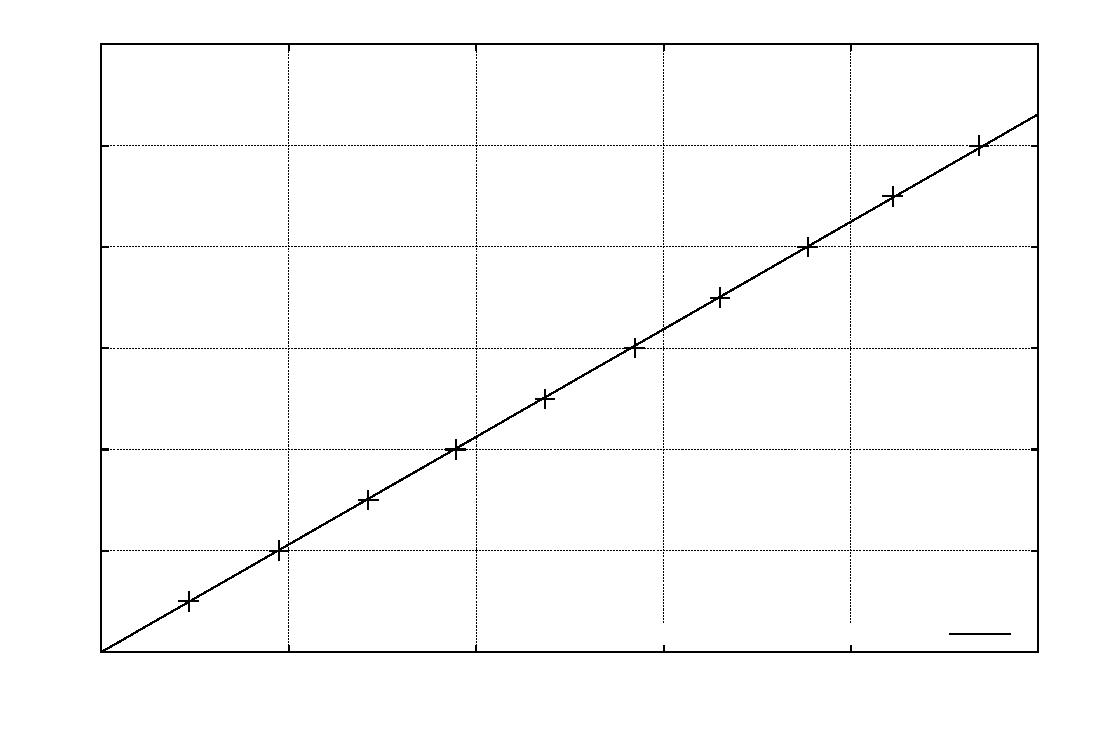
\includegraphics{vod}}%
    \gplfronttext
  \end{picture}%
\endgroup

\caption{Voltampérová charakteristika vzorku}
\label{g:vodivost}
\end{graph}


\begin{tabulka}[htbp]
\centering
\begin{tabular}{c||c|c|c|c||c|c|c|c}
& \multicolumn{4}{c||}{$I_{12}=\SI{2.50(6)}{\milli\ampere}$}  &  \multicolumn{4}{c}{$I_{12} = \SI{5.00(9)}{\milli\ampere}$} \\
$I_M (\si{\ampere})$ & $B (\si{\tesla})$ & $U_{56}^+ (\si{\milli\volt})$ & $U_{56}^- (\si{\milli\volt})$ & $U_H (\si{\milli\volt})$ & $B (\si{\tesla})$ & $U_{56}^+ (\si{\milli\volt})$ & $U_{56}^- (\si{\milli\volt})$  & $U_H (\si{\milli\volt})$ \\ \hline
\num{0.5} & \num{0.049} & \num{49} & \num{26} & \num{12} & \num{0.049} & \num{101} & \num{61}  & \num{20} \\
\num{1.0} & \num{0.098} & \num{59} & \num{14} & \num{23} & \num{0.098} & \num{123} & \num{38}  & \num{42} \\
\num{1.5} & \num{0.147} & \num{71} & \num{4} & \num{33} & \num{0.147} & \num{145} & \num{20}  & \num{63} \\
\num{2.0} & \num{0.196} & \num{82} & \num{-8} & \num{45} & \num{0.196} & \num{164} & \num{-2}  & \num{83} \\
\num{2.5} & \num{0.245} & \num{94} & \num{-17} & \num{55} & \num{0.245} & \num{187} & \num{-19}  & \num{103} \\
\num{3.0} & \num{0.294} & \num{104} & \num{-28} & \num{66} & \num{0.294} & \num{206} & \num{-41}  & \num{124} \\
\num{3.5} & \num{0.343} & \num{116} & \num{-37} & \num{76} & \num{0.343} & \num{230} & \num{-59}  & \num{145} \\
\num{4.0} & \num{0.392} & \num{126} & \num{-46} & \num{86} & \num{0.392} & \num{250} & \num{-77}  & \num{163} \\
\end{tabular}
\caption{Závislost Hallova napětí na magnetické indukci}
\label{t:hall}
\end{tabulka}

\begin{graph}[htbp]
\centering
% GNUPLOT: LaTeX picture with Postscript
\begingroup
  \makeatletter
  \providecommand\color[2][]{%
    \GenericError{(gnuplot) \space\space\space\@spaces}{%
      Package color not loaded in conjunction with
      terminal option `colourtext'%
    }{See the gnuplot documentation for explanation.%
    }{Either use 'blacktext' in gnuplot or load the package
      color.sty in LaTeX.}%
    \renewcommand\color[2][]{}%
  }%
  \providecommand\includegraphics[2][]{%
    \GenericError{(gnuplot) \space\space\space\@spaces}{%
      Package graphicx or graphics not loaded%
    }{See the gnuplot documentation for explanation.%
    }{The gnuplot epslatex terminal needs graphicx.sty or graphics.sty.}%
    \renewcommand\includegraphics[2][]{}%
  }%
  \providecommand\rotatebox[2]{#2}%
  \@ifundefined{ifGPcolor}{%
    \newif\ifGPcolor
    \GPcolorfalse
  }{}%
  \@ifundefined{ifGPblacktext}{%
    \newif\ifGPblacktext
    \GPblacktexttrue
  }{}%
  % define a \g@addto@macro without @ in the name:
  \let\gplgaddtomacro\g@addto@macro
  % define empty templates for all commands taking text:
  \gdef\gplbacktext{}%
  \gdef\gplfronttext{}%
  \makeatother
  \ifGPblacktext
    % no textcolor at all
    \def\colorrgb#1{}%
    \def\colorgray#1{}%
  \else
    % gray or color?
    \ifGPcolor
      \def\colorrgb#1{\color[rgb]{#1}}%
      \def\colorgray#1{\color[gray]{#1}}%
      \expandafter\def\csname LTw\endcsname{\color{white}}%
      \expandafter\def\csname LTb\endcsname{\color{black}}%
      \expandafter\def\csname LTa\endcsname{\color{black}}%
      \expandafter\def\csname LT0\endcsname{\color[rgb]{1,0,0}}%
      \expandafter\def\csname LT1\endcsname{\color[rgb]{0,1,0}}%
      \expandafter\def\csname LT2\endcsname{\color[rgb]{0,0,1}}%
      \expandafter\def\csname LT3\endcsname{\color[rgb]{1,0,1}}%
      \expandafter\def\csname LT4\endcsname{\color[rgb]{0,1,1}}%
      \expandafter\def\csname LT5\endcsname{\color[rgb]{1,1,0}}%
      \expandafter\def\csname LT6\endcsname{\color[rgb]{0,0,0}}%
      \expandafter\def\csname LT7\endcsname{\color[rgb]{1,0.3,0}}%
      \expandafter\def\csname LT8\endcsname{\color[rgb]{0.5,0.5,0.5}}%
    \else
      % gray
      \def\colorrgb#1{\color{black}}%
      \def\colorgray#1{\color[gray]{#1}}%
      \expandafter\def\csname LTw\endcsname{\color{white}}%
      \expandafter\def\csname LTb\endcsname{\color{black}}%
      \expandafter\def\csname LTa\endcsname{\color{black}}%
      \expandafter\def\csname LT0\endcsname{\color{black}}%
      \expandafter\def\csname LT1\endcsname{\color{black}}%
      \expandafter\def\csname LT2\endcsname{\color{black}}%
      \expandafter\def\csname LT3\endcsname{\color{black}}%
      \expandafter\def\csname LT4\endcsname{\color{black}}%
      \expandafter\def\csname LT5\endcsname{\color{black}}%
      \expandafter\def\csname LT6\endcsname{\color{black}}%
      \expandafter\def\csname LT7\endcsname{\color{black}}%
      \expandafter\def\csname LT8\endcsname{\color{black}}%
    \fi
  \fi
  \setlength{\unitlength}{0.0500bp}%
  \begin{picture}(10204.00,6802.00)%
    \gplgaddtomacro\gplbacktext{%
      \csname LTb\endcsname%
      \put(946,704){\makebox(0,0)[r]{\strut{} 0}}%
      \csname LTb\endcsname%
      \put(946,1390){\makebox(0,0)[r]{\strut{} 20}}%
      \csname LTb\endcsname%
      \put(946,2076){\makebox(0,0)[r]{\strut{} 40}}%
      \csname LTb\endcsname%
      \put(946,2763){\makebox(0,0)[r]{\strut{} 60}}%
      \csname LTb\endcsname%
      \put(946,3449){\makebox(0,0)[r]{\strut{} 80}}%
      \csname LTb\endcsname%
      \put(946,4135){\makebox(0,0)[r]{\strut{} 100}}%
      \csname LTb\endcsname%
      \put(946,4821){\makebox(0,0)[r]{\strut{} 120}}%
      \csname LTb\endcsname%
      \put(946,5508){\makebox(0,0)[r]{\strut{} 140}}%
      \csname LTb\endcsname%
      \put(946,6194){\makebox(0,0)[r]{\strut{} 160}}%
      \csname LTb\endcsname%
      \put(1078,484){\makebox(0,0){\strut{} 0}}%
      \csname LTb\endcsname%
      \put(2048,484){\makebox(0,0){\strut{} 0.05}}%
      \csname LTb\endcsname%
      \put(3018,484){\makebox(0,0){\strut{} 0.1}}%
      \csname LTb\endcsname%
      \put(3988,484){\makebox(0,0){\strut{} 0.15}}%
      \csname LTb\endcsname%
      \put(4958,484){\makebox(0,0){\strut{} 0.2}}%
      \csname LTb\endcsname%
      \put(5927,484){\makebox(0,0){\strut{} 0.25}}%
      \csname LTb\endcsname%
      \put(6897,484){\makebox(0,0){\strut{} 0.3}}%
      \csname LTb\endcsname%
      \put(7867,484){\makebox(0,0){\strut{} 0.35}}%
      \csname LTb\endcsname%
      \put(8837,484){\makebox(0,0){\strut{} 0.4}}%
      \csname LTb\endcsname%
      \put(9807,484){\makebox(0,0){\strut{} 0.45}}%
      \put(176,3620){\rotatebox{-270}{\makebox(0,0){\strut{}$U_H$ (\si{\milli\volt})}}}%
      \put(5442,154){\makebox(0,0){\strut{}$B$ (\si{\tesla})}}%
    }%
    \gplgaddtomacro\gplfronttext{%
      \csname LTb\endcsname%
      \put(3850,6278){\makebox(0,0)[r]{\strut{}$I_{12} = \SI{2.5}{\milli\ampere}$}}%
      \csname LTb\endcsname%
      \put(3850,5885){\makebox(0,0)[r]{\strut{}$U_H(\si{\milli\volt})=\num{223} \cdot B(\si{\tesla})$}}%
      \csname LTb\endcsname%
      \put(3850,5492){\makebox(0,0)[r]{\strut{}$I_{12} = \SI{5.0}{\milli\ampere}$}}%
      \csname LTb\endcsname%
      \put(3850,5099){\makebox(0,0)[r]{\strut{}$U_H(\si{\milli\volt})=\num{420} \cdot B(\si{\tesla})$}}%
    }%
    \gplbacktext
    \put(0,0){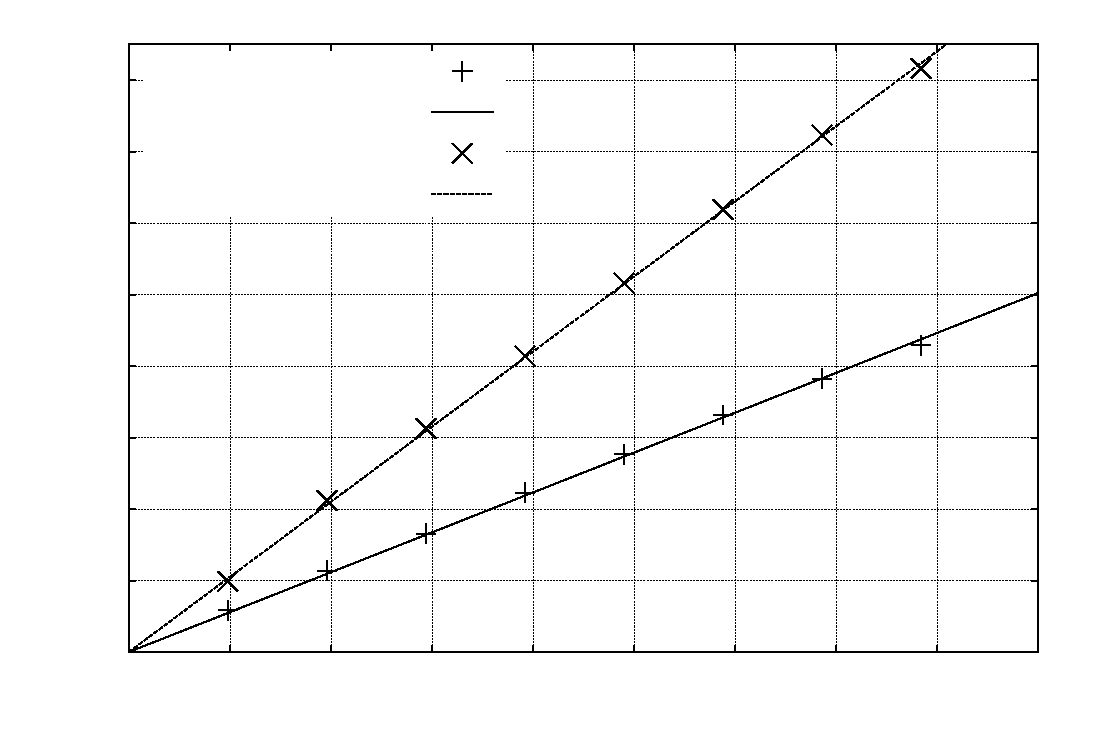
\includegraphics{hall}}%
    \gplfronttext
  \end{picture}%
\endgroup

\caption{Závislost Hallova napětí na magnetické indukci}
\label{g:hall}
\end{graph}